% Options for packages loaded elsewhere
\PassOptionsToPackage{unicode}{hyperref}
\PassOptionsToPackage{hyphens}{url}
%
\documentclass[
]{article}
\usepackage{amsmath,amssymb}
\usepackage{lmodern}
\usepackage{iftex}
\ifPDFTeX
  \usepackage[T1]{fontenc}
  \usepackage[utf8]{inputenc}
  \usepackage{textcomp} % provide euro and other symbols
\else % if luatex or xetex
  \usepackage{unicode-math}
  \defaultfontfeatures{Scale=MatchLowercase}
  \defaultfontfeatures[\rmfamily]{Ligatures=TeX,Scale=1}
\fi
% Use upquote if available, for straight quotes in verbatim environments
\IfFileExists{upquote.sty}{\usepackage{upquote}}{}
\IfFileExists{microtype.sty}{% use microtype if available
  \usepackage[]{microtype}
  \UseMicrotypeSet[protrusion]{basicmath} % disable protrusion for tt fonts
}{}
\makeatletter
\@ifundefined{KOMAClassName}{% if non-KOMA class
  \IfFileExists{parskip.sty}{%
    \usepackage{parskip}
  }{% else
    \setlength{\parindent}{0pt}
    \setlength{\parskip}{6pt plus 2pt minus 1pt}}
}{% if KOMA class
  \KOMAoptions{parskip=half}}
\makeatother
\usepackage{xcolor}
\IfFileExists{xurl.sty}{\usepackage{xurl}}{} % add URL line breaks if available
\IfFileExists{bookmark.sty}{\usepackage{bookmark}}{\usepackage{hyperref}}
\hypersetup{
  hidelinks,
  pdfcreator={LaTeX via pandoc}}
\urlstyle{same} % disable monospaced font for URLs
\usepackage[margin=1in]{geometry}
\usepackage{longtable,booktabs,array}
\usepackage{calc} % for calculating minipage widths
% Correct order of tables after \paragraph or \subparagraph
\usepackage{etoolbox}
\makeatletter
\patchcmd\longtable{\par}{\if@noskipsec\mbox{}\fi\par}{}{}
\makeatother
% Allow footnotes in longtable head/foot
\IfFileExists{footnotehyper.sty}{\usepackage{footnotehyper}}{\usepackage{footnote}}
\makesavenoteenv{longtable}
\usepackage{graphicx}
\makeatletter
\def\maxwidth{\ifdim\Gin@nat@width>\linewidth\linewidth\else\Gin@nat@width\fi}
\def\maxheight{\ifdim\Gin@nat@height>\textheight\textheight\else\Gin@nat@height\fi}
\makeatother
% Scale images if necessary, so that they will not overflow the page
% margins by default, and it is still possible to overwrite the defaults
% using explicit options in \includegraphics[width, height, ...]{}
\setkeys{Gin}{width=\maxwidth,height=\maxheight,keepaspectratio}
% Set default figure placement to htbp
\makeatletter
\def\fps@figure{htbp}
\makeatother
\setlength{\emergencystretch}{3em} % prevent overfull lines
\providecommand{\tightlist}{%
  \setlength{\itemsep}{0pt}\setlength{\parskip}{0pt}}
\setcounter{secnumdepth}{-\maxdimen} % remove section numbering
\ifLuaTeX
  \usepackage{selnolig}  % disable illegal ligatures
\fi

\author{}
\date{\vspace{-2.5em}}

\begin{document}

Table 1: Results of generalized linear mixed effect regression models
testing three measure of fire behavior against four potential predictor
variables. Statistics reflect pooled results of 50 imputed datasets
using the \emph{mice} package in R; see Methods. Vapor pressure deficit
included for Rate of spread only due to statistically-significant
difference between GLMM regression results that included VPD compared to
RH alone (Wald = 5.32, P = 0.02), while temperature models had no such
difference.

\begin{longtable}[]{@{}llrr@{}}
\toprule
Response & Model term & t df & P \\
\midrule
\endhead
Rate of spread & & & \\
& Wind speed & 2.92 108.0 & \textless{} 0.01 \\
& Vapor pressure deficit & -2.31 108.1 & 0.02 \\
& Relative humidity & -1.66 80.8 & 0.10 \\
& Fuel load & 1.16 49.9 & 0.25 \\
& Fuel moisture & -0.68 62.9 & 0.50 \\
Canopy temperature & & & \\
& Fuel load & 2.82 54.2 & 0.01 \\
& Fuel moisture & -2.16 40.9 & 0.04 \\
& Relative humidity & -1.19 120.4 & 0.24 \\
& Wind speed & 0.02 132.4 & 0.99 \\
Surface temperature & & & \\
& Relative humidity & -1.19 74.8 & 0.24 \\
& Fuel load & -0.48 20.1 & 0.64 \\
& Fuel moisture & -0.47 40.1 & 0.64 \\
& Wind speed & 0.06 49.5 & 0.95 \\
\bottomrule
\end{longtable}

Figure 1: Distribution of weather, fuel, and fire behavior data for
fires in southwestern North Dakota (Hettinger, dark maroon) and central
North Dakota (Central Grasslands, light blue). Horizontal gray lines
denote 25\%, 50\% (median) and 75\% quantiles; triangles are arithmetic
means. Means and standard deviation are also reported in Supplemental
Information Table 1. VPD = Vapor pressure deficit.
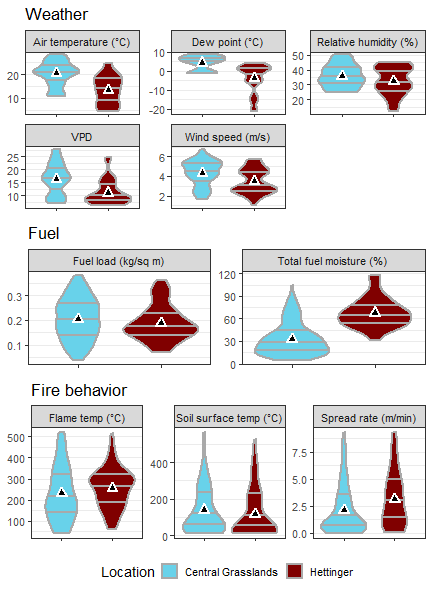
\includegraphics{./springer/data_summary_gg-1.png}

\newpage

Figure 2: Principal Components Analysis of fire behavior data (response
variables in blue; rate of spread (ROS), temperature above surface
(flame ºC), and temperature at soil surface (soil ºC) for prescribed
burns on rangeland at Hettinger (H), in southwestern North Dakota, and
Central Grasslands (CG), in central North Dakota. No difference between
locations (P = 0.11). Total variance explained in these two axes = 86\%.
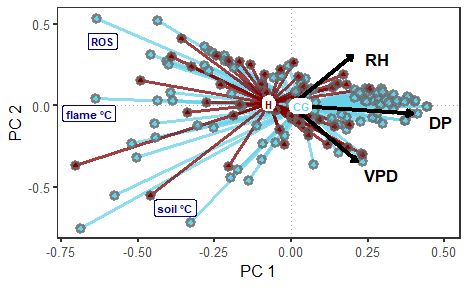
\includegraphics{./springer/pca_gg-1.png}

\newpage

Figure 3: Regression coefficients and 95\% confidence intervals for fuel
and weather terms from models for maximum temperature at 15 cm above the
soil surface (flame), maximum temperature at the soil surface (soil),
and rate of spread. 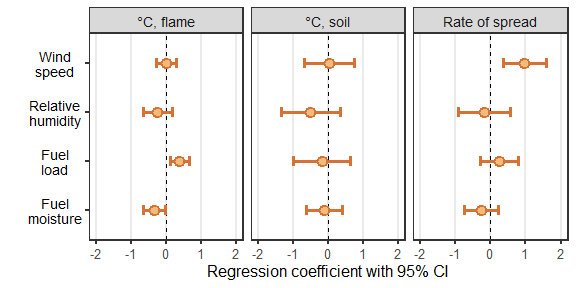
\includegraphics{./springer/CI_gg-1.png}

\end{document}
